\documentclass{beamer}

\usepackage[utf8]{inputenc}
\usepackage[T1]{fontenc}
\usepackage[francais]{babel}
\usepackage{movie15}

\usetheme{Darmstadt}
\usecolortheme{seahorse}
%\setbeamertemplate{footline}[frame number]
\setbeamertemplate{footline}{
    \leavevmode%
    \hbox{\hspace*{-0.06cm}
        %\begin{beamercolorbox}[wd=.2\paperwidth,ht=2.25ex,dp=1ex,center]{author in head/foot}%
        %\usebeamerfont{author in head/foot}\insertshortauthor%~~(\insertshortinstitute)
        %\end{beamercolorbox}%
        \begin{beamercolorbox}[wd=.8\paperwidth,ht=2.25ex,dp=1ex,center]{section in head/foot}%
            \usebeamerfont{section in head/foot}\insertshorttitle
        \end{beamercolorbox}%
        \begin{beamercolorbox}[wd=.2\paperwidth,ht=2.25ex,dp=1ex,right]{section in head/foot}%
            \usebeamerfont{section in head/foot}\insertshortdate{}\hspace*{2em}
            \insertframenumber{} / \inserttotalframenumber\hspace*{2ex}
    \end{beamercolorbox}}%
    \vskip0pt%
}

\usepackage{graphicx}

\AtBeginSection[]{
    \begin{frame}
        \frametitle{Plan}
        \tableofcontents[currentsection,hideothersubsections]
    \end{frame} 
}

\titlegraphic{
    \begin{columns}
        \column{.1\textwidth}
        
\includegraphics[width=\textwidth]{img/imag.eps}
        \column{.4\textwidth}
        
\includegraphics[width=\textwidth]{img/topSolid.eps}
    \end{columns}
}

\title{Simulation de pliage dans un outillage progressif}
\author{Ariane LEFEBVRE \and Pablo COVES\\[.5cm] Master 2 MIA Image et CAO \and 2012-2013\\[.5cm] Tuteurs: Christophe PICARD \and Frédéric PONTAROLLO}
\date{}

\begin{document}
\maketitle

\section{Introduction}
\subsection{Missler Software}
\begin{frame}
    \begin{itemize}
        \item Première solution CFAO dans les années 80.
        \item Les services TopSolid:
            \begin{itemize}
                \item Générale: modélisation, assemblage...
                \item Outillage: moules, matrices...
                \item Tôlerie: Design, découpe et mise-en-forme.
            \end{itemize}
    \end{itemize}
\end{frame}
\subsection{Outillage progressif}
\begin{frame}
    \begin{columns}
        \column{.3\textwidth}
        \begin{itemize}
            \item Poinçon.
            \item Dévêtisseur.
            \item Tôle.
            \item Matrice.
        \end{itemize}
        \column{.7\textwidth}
        \begin{figure}
            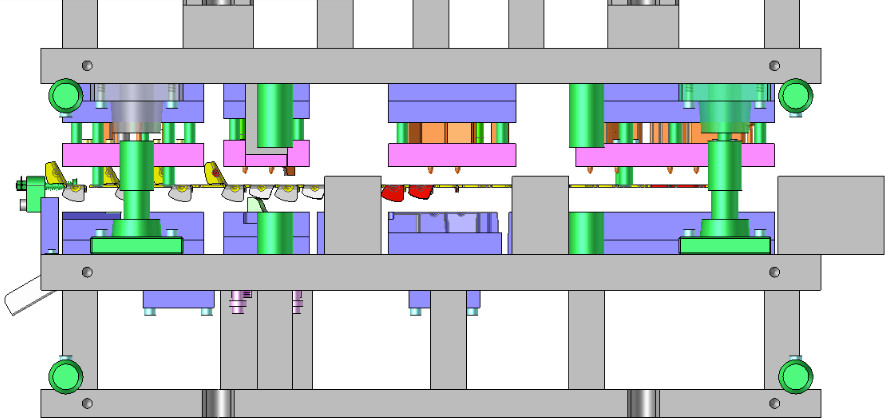
\includegraphics[width=\textwidth]{img/dieTool.jpg}
            \caption{Outillage progressif}
        \end{figure}
    \end{columns}
\end{frame}
\subsection{Opérations de base}
\begin{frame}
    \begin{itemize}
        \item Découpe:\\
            Ôte des morceaux des matériaux.
        \item Pliage:\\
            Modification de la forme de la tôle par formation d'angles.
        \item Poinçonnage:\\
            Forte pression provoquant une déformation.
    \end{itemize}
\end{frame}

\section{Contenu du projet}
\subsection{Projet du client}
\begin{frame}
    \frametitle{Spécifications}
    \begin{itemize}
        \item Application pour simuler en 2D une déformation réaliste.
        \item Retour élastique au retour du poinçon.
        \item Aire couverte par la tôle.
        \item Suivit d'un point en temps réel.
    \end{itemize}
\end{frame}
\begin{frame}
    \frametitle{Représentation 2D}
    \begin{columns}
        \column{.6\textwidth}
        \begin{itemize}
            \item \textbf{La matrice}: 
                Un polygone, fixe au cours du temps.
            \item \textbf{Le dévêtisseur}:
                Un polygone venant fixer la tôle à la matrice.
            \item \textbf{Le poinçon}:
                Un polygone en mouvement. Il vient frapper la tôle.
            \item \textbf{La tôle}:
                D'épaisseur fixe, elle est décrite par sa fibre neutre.
        \end{itemize}
        \column{0.4\textwidth}
        \begin{figure}
            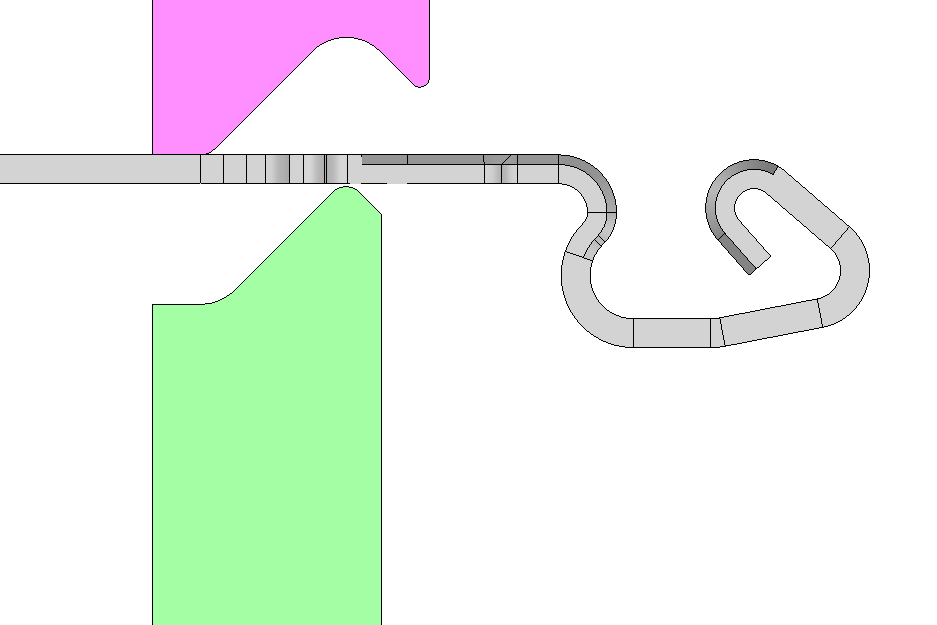
\includegraphics[width=\textwidth]{img/fibreNeutre.jpg}
            \caption{Représentation 2D}
        \end{figure}
    \end{columns}
\end{frame}
\subsection{Tâches à réaliser}
\subsubsection{Interface utilisateur}
\begin{frame}
    \frametitle{Interface utilisateur}
    Une fenêtre contenant:
    \begin{itemize}
        \item Des menus déroulant: choix des intéractions souris.
        \item Pas de temps entre chaque étapes.
        \item Temps totale de la simulation.
        \item Un lecteur pour la visualisation.
        \item Une zone de rendu OpenGL.
    \end{itemize}
\end{frame}
\subsubsection{Chargement d'une scène}
\begin{frame}
    \frametitle{Chargement d'une scène}
    Une scène est décrite par un fichier XML:
    \begin{itemize}
        \item Fourni par le client.
        \item Contient les caractéristiques du matériau.
        \item Contient les positions des éléments fixes.
        \item Contient les positions hautes et basses du poinçon.
    \end{itemize}
\end{frame}
\subsubsection{Moteur de déformations}
\begin{frame}
    \frametitle{Le moteur de déformation}
    \begin{figure}
        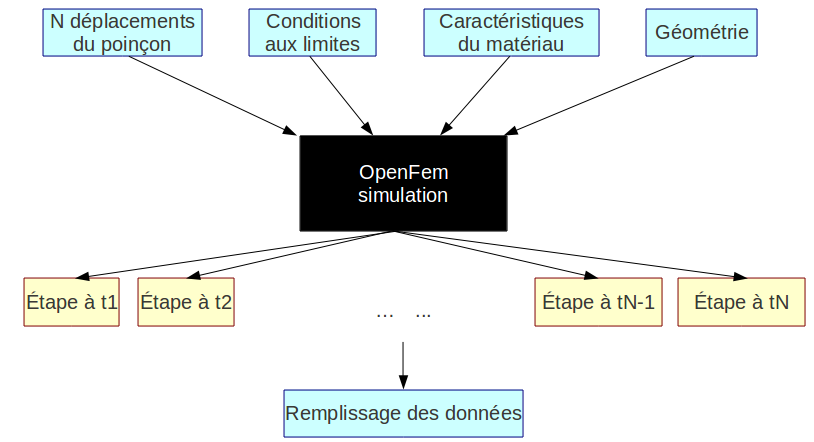
\includegraphics[width=\textwidth]{img/OpenFEM.png}
        \caption{Dialogue avec le moteur de déformation}
    \end{figure}
\end{frame}
\subsection{Liste des livrables}
\begin{frame}
    Concernant la partie Image et CAO:
    \begin{itemize}
        \item Visualisation grâce au lecteur sous forme d'une vidéo ou étape par étape.
        \item Deux intéractions à la souris.
        \item Affichage de l'aire couverte par la tôle.
    \end{itemize}
\end{frame}

\section{Description des méthodes}
\subsection{Méthodologie générale}
\begin{frame}
    \frametitle{Architecture}
    \begin{itemize}
        \item Modèle MVC.
        \item Librairie graphique Qt.
        \item Multi-plateforme.
    \end{itemize}
\end{frame}
\subsection{Méthodes envisagées ou utilisées}
\begin{frame}
    \frametitle{Méthodes envisagées}
    \begin{columns}
        \column{.6\textwidth}
        \begin{itemize}
            \item Affichage de formes complexes.
                \begin{itemize}
                    \item Polygones concaves.
                    \item Polygones avec auto-intersections.
                \end{itemize}
            \item Nécesite:
                \begin{itemize}
                    \item Concavité $\rightarrow$ triangulation.
                    \item Intersection $\rightarrow$ nouveau polygone.
                \end{itemize}
        \end{itemize}
        \column{.4\textwidth}
        \begin{figure}
            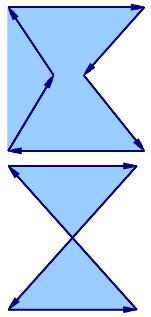
\includegraphics[width=.5\textwidth]{img/concave.png}
            \caption{Formes complexes}
        \end{figure}
    \end{columns}
\end{frame}
\begin{frame}
    \frametitle{Méthodes utilisées}
    %Déplacement du poinçon: bielle-manivelle $\rightarrow$ vitesse variable.
    \begin{center}
        $P(t) = \frac{-Dmax}{2}*\cos(\frac{2}{Tmax}*\pi*t)+\frac{Dmax}{2}$
    \end{center}
    \begin{figure}
        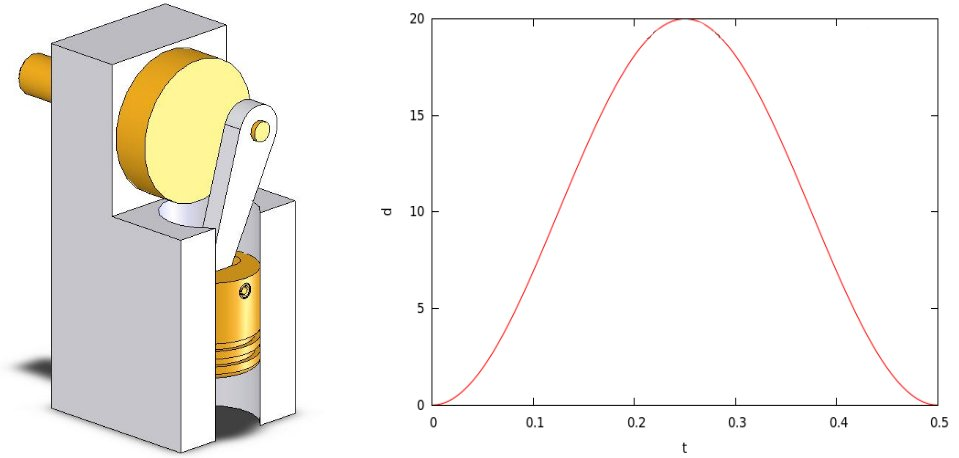
\includegraphics[width=.7\textwidth]{img/bielle.jpg}
        \caption{Système bielle-manivelle}
    \end{figure}
\end{frame}


\section{Résultats}
\subsection{Expérimentations réalisées}
\begin{frame}
    \frametitle{Procédés de validation}
    \begin{figure}
        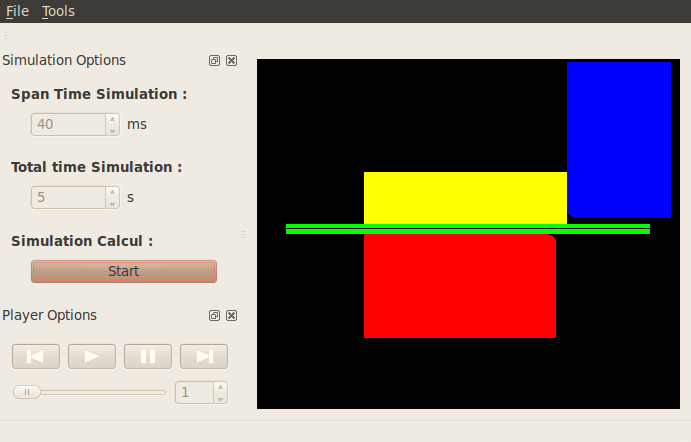
\includegraphics[width=.45\textwidth]{img/fenetreInitiale.png}$~~~$
        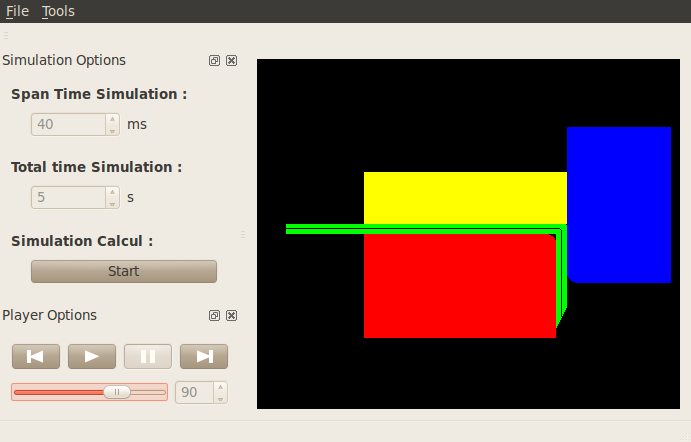
\includegraphics[width=.45\textwidth]{img/fenetreInitiale2.png}
        \caption{Tests unitaires}
    \end{figure}
\end{frame}
\begin{frame}
    \frametitle{Suivi de point}
    \begin{figure}
        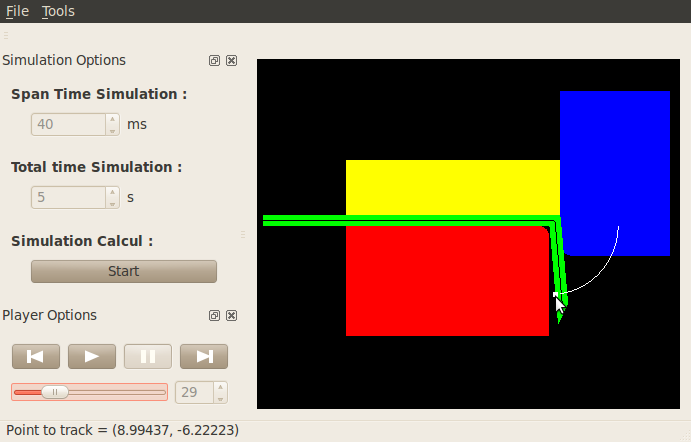
\includegraphics[width=.8\textwidth]{img/tracking.png}
        \caption{Trajectoire d'un point de la tôle}
    \end{figure}
\end{frame}
\begin{frame}
    \frametitle{Distance entre deux points}
    \begin{figure}
        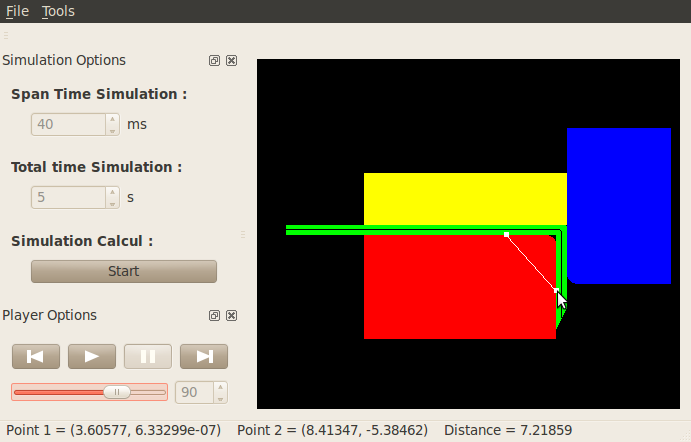
\includegraphics[width=.8\textwidth]{img/distance.png}
        \caption{Distance entre deux points}
    \end{figure}
\end{frame}
\begin{frame}
    \frametitle{Aire de couverture}
    \begin{figure}
        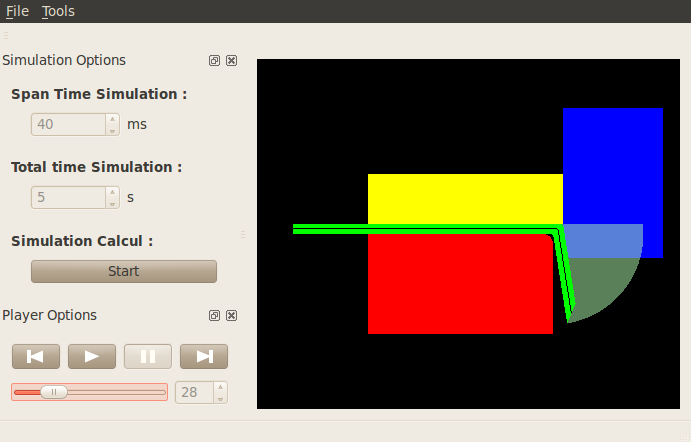
\includegraphics[width=.8\textwidth]{img/area.png}
        \caption{Aire couverte par la tôle}
    \end{figure}
\end{frame}
\begin{frame}
    \frametitle{Démonstration}
    \begin{center}
        \includemovie[attach=true,autoplay]{217pt}{162pt}{Pliage.mov}
    \end{center}
\end{frame}
\subsection{Évaluation des résultats}
\begin{frame}
    \frametitle{Qualité des résultats}
    \begin{itemize}
        \item Le rendu:
            \begin{itemize}
                \item Lecteur opérationel et robuste.
                \item Durée et pas de temps fixes.
            \end{itemize}
        \item Suivi d'un point:
            \begin{itemize}
                \item Modifiable en cours de simulation.
                \item Affichage en temps réel.
                \item Coordonées réelles.
            \end{itemize}
    \end{itemize}
\end{frame}
\begin{frame}
    \frametitle{Qualité des résultats}
    \begin{itemize}
        \item Distance entre deux points:
            \begin{itemize}
                \item Affichage dans la barre de status.
                \item Coordonées réelles.
                \item Limite: translation.
            \end{itemize}
        \item Aire de couverture:
            \begin{itemize}
                \item Temps réel.
                \item Transparence.
            \end{itemize}
    \end{itemize}
\end{frame}
\subsection{Critiques et commentaires}
\begin{frame}
    \frametitle{Critiques et commentaires}
    \begin{itemize}
        \item Les plus:
            \begin{itemize}
                \item Spécification Image et CAO remplies.
                \item Mouvement du poinçon réaliste.
                \item Peut fonctionner sur des simulations réalistes.
            \end{itemize}
        \item Les moins:
            \begin{itemize}
                \item Formes complexes.
                \item Moteur de déformation $\rightarrow$ Cas particulier.
            \end{itemize}
    \end{itemize}
\end{frame}

\section{Conclusion}
\begin{frame}
    \frametitle{Conclusion}
    \begin{itemize}
        \item Absence du membre MCS.
        \item Séparation nette dans l'application.
        \item Relation avec le client.
    \end{itemize}
\end{frame}
\subsection{Diagrammes de Gantt}
\begin{frame}
    \frametitle{Plan initial}
    \begin{figure}
        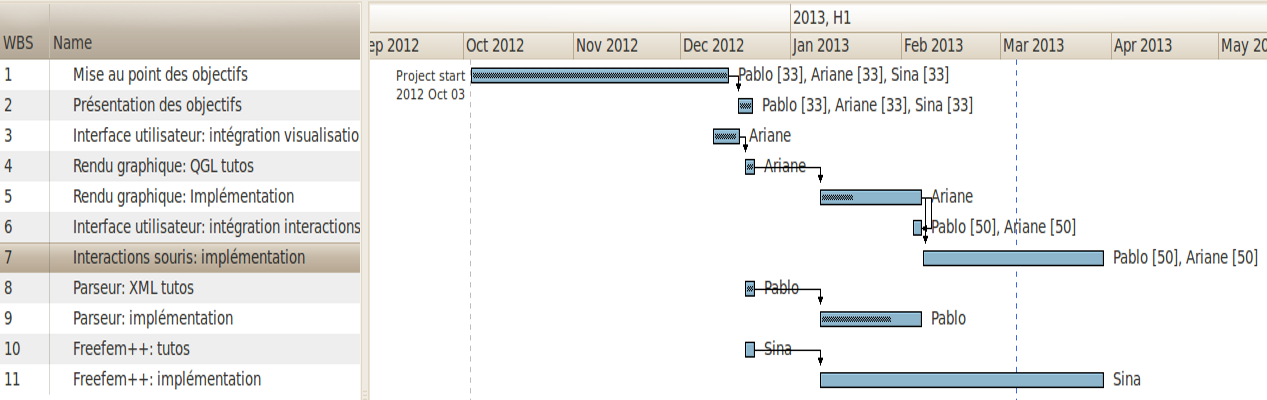
\includegraphics[width=\textwidth]{img/gantt.png}
        \caption{Répartition initiale}
    \end{figure}
\end{frame}
\begin{frame}
    \frametitle{Fin de projet}
    \begin{figure}
        \includegraphics[width=\textwidth]{img/ganttFin.png}
        \caption{Répartition en fin de projet}
    \end{figure}
\end{frame}
\subsection{Perspectives}
\begin{frame}
    \frametitle{Perspectives}
    \begin{itemize}
        \item Faire varier l'épaisseur de la tôle.
        \item Triangulation pour les formes complexes.
        \item Intégrer le moteur de déformations.
    \end{itemize}
\end{frame}
\subsection{Questions}
\begin{frame}
    \frametitle{Questions}
    Merci pour votre attention\\[3.5cm]
    \hfill Des questions?
\end{frame}


\end{document}
